\documentclass[11pt, oneside]{article} 
\usepackage{geometry}
\geometry{letterpaper} 
\usepackage{graphicx}
	
\usepackage{amssymb}
\usepackage{amsmath}
\usepackage{parskip}
\usepackage{color}
\usepackage{hyperref}

\graphicspath{{/Users/telliott_admin/Dropbox/Tex/png/}}
% \begin{center} 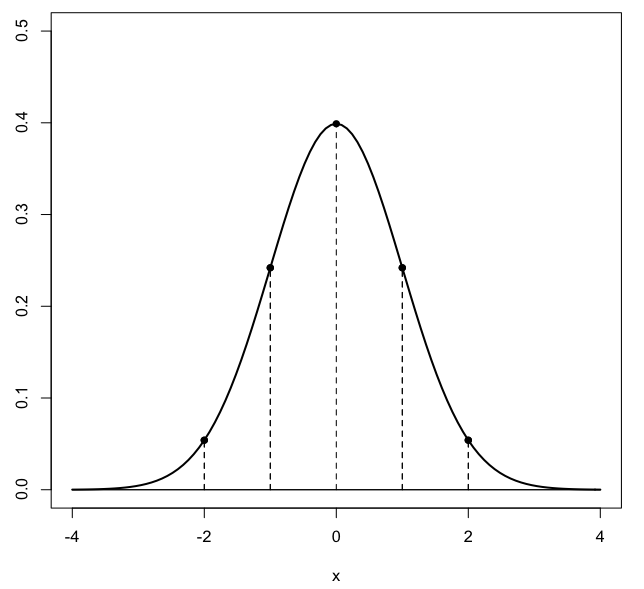
\includegraphics [scale=0.4] {gauss3.png} \end{center}

\title{Newton point mass}
\date{}

\begin{document}
\maketitle
\Large

\label{sec:Newton_point_mass}

In this chapter, we explore Newton's famous result, that the mass of a spherical body behaves in terms of gravitational attraction as if it were concentrated at the center of the sphere.  
We adopt the notation shown below as the standard for the discussion of this theorem in this chapter and the next.  A point mass $m$ (blue circle) lies at a distance $D$ from the center of a sphere.
\begin{center} 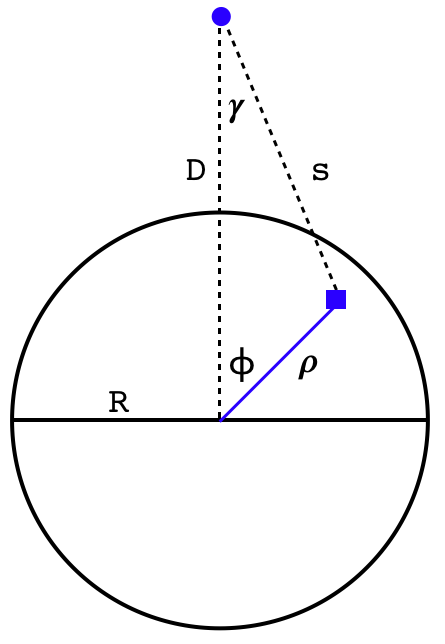
\includegraphics [scale=0.35] {newton_volume.png} \end{center}
For some reason, both Strang and Kline use $D$ for the distance to the center of the sphere, and I have kept that.  Keep your eye on $D$.  The sphere has mass $M$ and radius $R$.

For the radial segment to the volume element (or the part of a spherical belt, next chapter) I have adopted $\rho$ from Strang, while $s$ is the distance from the volume element to the test mass $m$.  The inverse square law says that the force varies like $1/s^2$ for each little mass element $dM$ contained in a little volume element $dV$.

We are free to choose the coordinate system;  a convenient choice is to orient the $z$-axis so that $m$ lies along a ray out along $z$ and the ray to any little volume element $dV$ (blue square) makes the usual polar angle $\phi$ as shown.  We also need the angle $\gamma$ shown in the figure.
\begin{center} 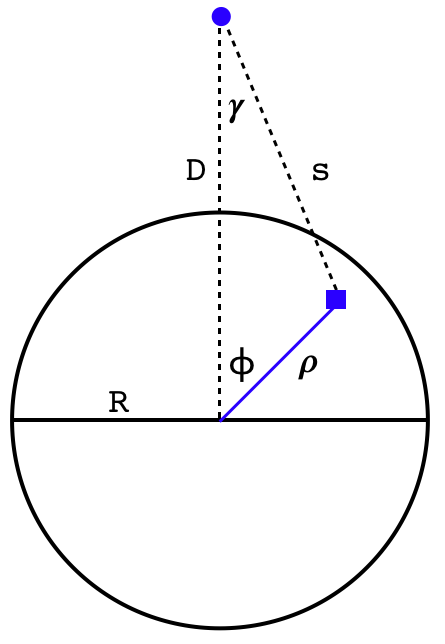
\includegraphics [scale=0.3] {newton_volume.png} \end{center}
There are two different ways of setting up the integral.  One, as indicated by use of $dV$, is to do a triple integral over the volume, using spherical coordinates.  For this approach, we integrate first over $\phi$, then over $\rho$ and finally add $2 \pi$ from the radial angle $\theta$, which is the outer integral.

An alternative approach is to consider a hollow shell.  We first prove that the shell acts as if its mass were at the center, then layers of concentric shells all add up to the total result.  The shell approach is not really all that different from the volume integral.

The important difference between the two approaches is that Kline (shell theorem, next chapter) uses $s$ as a variable of integration.  This unique approach gives an easy extension to a result that we have already used in the book.

Going on then with the first approach, the force on the point mass due to the volume element is $mG/s^2 \cdot dM$ where $dM = M/V \ dV$.  Thus, we will have a constant factor of $mMG$ divided by the volume of the sphere multiplying the result.  We leave this to one side for now.  If you don't follow this, take a look at the longer explanation in the \hyperref[sec:Newton]{\textbf{appendix}}.

The interesting part of the integral comes from understanding that $s^2$ depends on where the volume element is located, and second, the force, which acts in the direction of $s$, has a sideways component $F \sin \gamma$ that cancels by radial symmetry, and a vertical component $F \cos \gamma$, which does not cancel.

Thus, to get the force, we have our remembered constant times the integral:
\[ \int_V \frac{1}{s^2} \cos \gamma \ dV \]
\[ = \iiint  \ [ \frac{1}{s^2} \cos \gamma \ ] \ \rho^2 \sin \phi \ d \rho \ d \phi \ d \theta \]

It turns out that these two effects (of $1/s^2$ and $\cos \gamma$) cancel, so that the value of the integral is $1/D^2 \cdot V$.  

\subsection*{doing the integral}
The inner integral is taken with respect to $\phi$ (holding $\theta$ and $\rho$ constant).  
\[ I = \int  \ [ \frac{1}{s^2} \cos \gamma \ ] \ \rho^2 \sin \phi \ d \phi  \]
We come up against the problem that $s$ and $\gamma$ are themselves both variables.  To make progress, we must express everything in terms of the single variable, $\phi$.
\begin{center} 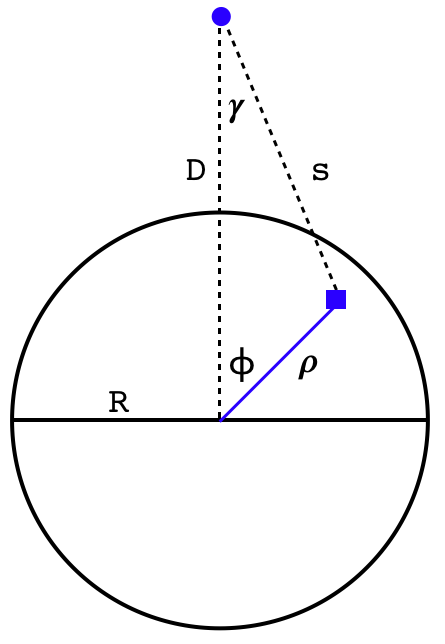
\includegraphics [scale=0.3] {newton_volume.png} \end{center}

We use the law of cosines twice.  First,
\[ s^2 = D^2 + \rho^2 - 2 D \rho \cos \phi \]
Second
\[ \rho^2 = D^2 + s^2 - 2Ds \cos \gamma \]
\[ \cos \gamma = \frac{D^2 + s^2 - \rho^2}{2Ds} \]
For simplicity, we substitute only for $\cos \gamma$ and not yet for $s^2$ 
\[ I = \int \frac{1}{s^2} \ [ \  \frac{D^2 + s^2 - \rho^2}{2Ds}  \ ] \ \rho^2 \sin \phi \ d \phi \]
Even with that restraint, I think we can agree that this looks like a bit of a mess.  

But now we have an inspiration! Make the substitution:
\[ u = s^2 = D^2 + \rho^2 - 2 D \rho \cos \phi \]
The derivative
\[ du = 2 D \rho \sin \phi \ d \phi \]
\[ \rho \sin \phi \ d \phi = \frac{1}{2D} \ du \]

With the substitution we generate a factor of $\sin \phi$ and can see a path forward:
\[ I = \int \frac{1}{s^2} \ [ \  \frac{D^2 + s^2 - \rho^2}{2Ds}  \ ] \ \rho^2 \sin \phi \ d \phi \]
\[ = \int \frac{1}{u} \cdot \frac{u + D^2 - \rho^2}{2D \sqrt{u}} \cdot \rho \cdot \frac{1}{2D} \ du\]
\[ = \frac{\rho}{4D^2} \int \frac{u + D^2 - \rho^2}{u^{3/2}} \ du \]
The integral breaks into two parts which are pretty easy
\[  = \frac{\rho}{4D^2} \ [ \  \int \frac{1}{\sqrt{u}} \ du + \int \frac{D^2 - \rho^2}{u^{3/2}} \ du \ ]  \]
\[ = \frac{\rho}{4D^2} \ [ \ 2 \sqrt{u} - 2 \ \frac{D^2 - \rho^2}{\sqrt{u}}  \ ] \]
\[ = \frac{\rho}{2D^2} \ [ \ \sqrt{u} - \ \frac{D^2 - \rho^2}{\sqrt{u}}  \ ] \]

Now, we reverse the substitution, but do it gradually.  Think about
\[ u = s^2 = D^2 + \rho^2 - 2 D \rho \cos \phi \]
The bounds on $\phi$ are the usual $[0,\pi]$  At the upper bound $\cos \phi = -1$ and
\[ u = D^2 + \rho^2 + 2 D \rho = (D + \rho)^2 \]
\[ \sqrt{u} = D + \rho \]
So the term in brackets is 
\[ \sqrt{u} - \ \frac{D^2 - \rho^2}{\sqrt{u}} = D + \rho - \frac{(D + \rho)(D - \rho)}{D + \rho} = 2 \rho \]
You don't see that kind of simplification every day!

At the lower bound, $\cos \phi = 1$ and
\[ u = D^2 + \rho^2 - 2 D \rho = (D - \rho)^2 \]
\[ \sqrt{u} = D - \rho \]
The term in brackets is
\[ = D - \rho - \frac{(D + \rho)(D - \rho)}{D - \rho} = - 2 \rho \]
but we are subtracting the value at the lower bound, so in the end the terms in the brackets add up to $4 \rho$ and the whole integral is
\[ I = \frac{\rho}{2D^2} \cdot 4 \rho = 2 \frac{\rho^2}{D^2} \]

We integrate next over $\rho$ and obtain
\[ \frac{2}{D^2} \int_0^R \rho^2 \ d \rho = \frac{2}{D^2} \ \frac{R^3}{3} \]
Finally, we pick up $2 \pi$ from the outer integral:
\[ \frac{4/3 \ \pi R^3}{D^2}  = \frac{V}{D^2}  \]

Recall that we left aside a constant factor of $mMG$ divided by the volume $V$.  Hence the force is:
\[ F = \frac{mMG}{D^2}  \]

The essence of our result is that
\[ \int_V \frac{1}{s^2} \cos \gamma \ dV = \frac{V}{D^2}  \]
The \emph{average value} of the function $1/s^2 \ \cos \gamma$ taken over the whole sphere is the above divided by $V$ or just $1/D^2$.  
\begin{center} 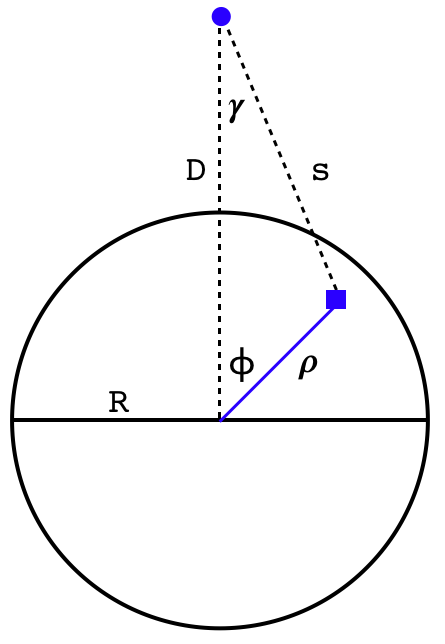
\includegraphics [scale=0.35] {newton_volume.png} \end{center}
Remarkable.

\end{document}